\documentclass{../../../lessonplan}
\renewcommand{\cflroot}{../../..}

\begin{document}

\lessonplantitle
    {KS1-S1}
    {Key Stage 1 Session 1}
    {Unplugged algorithms for moving along a route}

\preamble
    {
    \item Understand that an algorithm is a set of instructions a particular order
    \item Create a set of instructions navigate a simple route, using forwards, left, and right commands
    \item Follow a set of instructions accurately
    \item Record instructions accurately
    }
    {
    \item Print and cut out van cards and arrow direction cards from KS1 assets
    \item Resource sheets KS1-S1-1 to KS1-S1-3 (enough for each pair to have two sheets)
    \item Resource sheet KS1-S3-4, with a van card cut out and stuck on to a cube (e.g.\ Dienes unit)
    \item If working with a large group or entire class, you could make a large grid mat and print a large version of the van onto card.
               Attach the image of the van on top of a toy car so that it can easily move around the grid.
    }
    {
    \item Instructions, sequence, algorithm
    \item Forward, backward, right, left, corner
    \item Route, journey
    }

\begin{lessonplan}

Talk to the children about delivery vans.
Have they seen any? (Royal Mail, DHL, Ocado etc.)

In this project they are going to control their own van on the computer.

They will control the van by giving it instructions to move.
Very clear instructions.

Explain the learning expectations and that they will be computer programmers, but before that they will look at a model of a van on a tabletop map to think about how to give it clear instructions.

Demonstrate how the van travels along the road on resource sheet KS1-S1-1 \textit{[fig S1.1]}.

\fig{fig S1.1}{figS1.1.jpg}{1}

\keyquestion{What types of movement is it making?} (e.g.\ moving forwards, driving around a corner)

\keyquestion{If we are going to give exact instructions, what might those instructions be?}

\keyquestion{If we just say go forward, exactly how far forward do we mean?}

Guide the discussion so that the children understand that `drive forward one grid square' is more precise that `move forward', and that `drive around the corner to the right' is clearer than `go that way'!

\fig{fig S1.2}{figS1.2.jpg}{1}

Explain how the children are going to use the arrow direction cards \textit{[fig S1.2]} to record their instructions.
Explain that the rules for this van are a little different from a BeeBot.
Forward means one grid square from edge to edge.
Turn right means drive around the corner to the right from edge to edge \textit{[fig S1.3]}.

\fig{fig S1.3}{figS1.3.jpg}{1}



\subsection*{Explain the activity}

Sitting on the floor, ask one child to mvoe the van card and say the instruction that is being followed, e.g.\ \keyword{forward}.

Ask another child to choose an arrow direction card to record this.

Demonstrate this step-by-step, so that you end up with a short sequence of arrow cards e.g.\

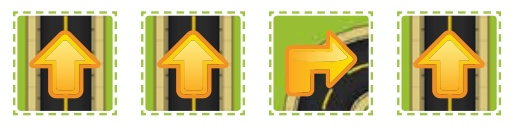
\includegraphics[width=.667\linewidth]{arrow_cards.jpg}

Get the children to say the sequence out loud \textit{[fig S1.4]}.  \fig{fig S1.4}{figS1.4.jpg}{1}

If some children are having difficulting distinguishing left from right, try using the Left and Right van cards in the Assets file.


\subsection*{Key questions}

\keyquestion{Does it matter in which order we give the instructions?}

\keyquestion{What would happen if we mixed them up?}

Explain that a sequence of instructions in the correct order to drive the van from start to finish is called an \keyword{algorithm}.


\subsection*{Paired activity}

Give each pair of children resource sheet KS1-S1-4, a van card and a set of arrow direction cards to record the route.
One child can be the `driver' one can be the `tracker'.

Explain that the `driver' takes the fan from the start point to the finish point, and tells the `tracker' what each instruction is.
The `tracker' records the journey using the arrow cards.

Change roles, repeat activity.



\subsection*{Mini review}

Bring the group back together and ask on pair to show their route and instructions.
Ask another child to lest out the instructions by following them from the start point.

Demonstrate how they could record this on a mini whiteboard instead of using the cards.

Give each pair a chance to do the same activity with the next grid route, this time recording the movement on their whiteboards or on KS1-S1-2 to KS1-S1-4 \textit{[fig S1.5]}, drawing their own arrow instructions, or if they prefer, using F, R and L.

\fig{fig S1.5}{figS1.5.jpg}{1}

\end{lessonplan}

\end{document}
